\documentclass[12pt, a4paper]{article}

\usepackage[T1]{fontenc}
\usepackage{courier}
\usepackage{graphicx}
\usepackage{caption}
\usepackage{mathptmx}
\usepackage{ragged2e}
\usepackage{xcolor}
\usepackage{listings}
\usepackage{enumitem}

\graphicspath{{img}}
\pagenumbering{gobble}
\date{}

\captionsetup[figure]{labelformat=empty}

\begin{document}

    NAMA: RADINAL SHIDIQ SARAGIH

    KELAS: IF C 2023

    NPM: 5520123104

  \begin{center}
    \section*{Laporan Konfigurasi Static Routing di GNS-3}
  \end{center}

  \begin{figure}[h]
      \centering
      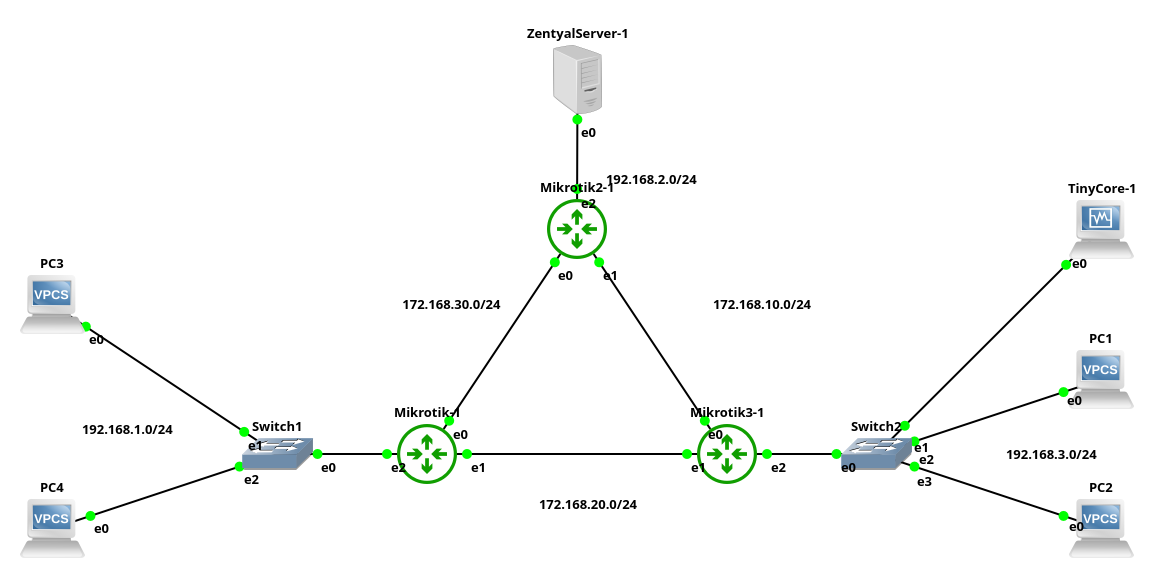
\includegraphics[scale=0.4]{TOPOLOGI.png}
  \end{figure}

  Disini terdapat sebuah topologi jaringan komputer, dimana didalamnya
  terdapat tiga buah router yang menghubungkan tiga jaringan yang berada
  di net id yang berbeda. Untuk mengkonfigurasi topologi ini pertama yang
  perlu dilakukan ada mengkonfigurasi alamat IP.

  Pada topologi diatas, dapat dilihat bahwa koneksi antar router
  dilakukan melalui interface serial, dan tiap router memiliki dua kabel
  serial yang terhubung ke router lainnya, dan selain serial terdapat
  sebuah interface Ethernet yang akan terhubung
  pada sebuah switch. Maka dari Gambar diatas untuk tiap router akan
  memerlukan tiga buah alamat IP.

  Untuk mengkonfigurasi IP sebuah interface router dapat dilakukan melalui
  tampilan terminal router.
  
  \begin{figure}[h]
      \centering
      \includegraphics[scale=0.4]{R1\_CONF\_IP\_TABLE\_PRE.png}
  \end{figure}

  Setelah membuka tampilan terminal sebuah router, hal pertama yang
  perlu dilakukan adalah melihat interface apa saja yang tersedia pada router
  tersebut dengan menggunakan perintah seperti di gambar diatas.

  Pada router "R1" dapat dilihat bahwa router tersebut memiliki 2 buah 
  interface Ethernet dan 4 buah Interface Serial.

  Setelah mengetahui informasi tentang jumlah dan status dari semua
  interface jaringan yang tersedia, sekarang yang perlu dilakukan adalah
  untuk memberikan interface-interface yang akan digunakan sebuah alamat
  IP.

  Dalam topologi yang digunakan disini hanya akan memanfaatkan interface 
  FastEthernet0/0, Serial 1/0 dan Serial1/1. Untuk mengkonfigurasi ketiga
  interface tersebut dapat dilakukan sebagai berikut.

  \begin{enumerate}
    \item Interface FastEthernet0/0
      \begin{center}
        \includegraphics[scale=0.4]{R1\_CONF\_IP\_FA.png}
      \end{center}

    \item Interface Serial1/0
      \begin{center}
        \includegraphics[scale=0.4]{R1\_CONF\_IP\_S10.png}
      \end{center}

    \item Interface Serial1/1
      \begin{center}
        \includegraphics[scale=0.4]{R1\_CONF\_IP\_S11.png}
      \end{center}
  \end{enumerate}
Lalu untuk memastikan IP telah ditetapkan dengan benar, bisa dilakukan dengan perintah sebagai berikut.

  \begin{figure}[h]
      \centering
      \includegraphics[scale=0.4]{R1\_CONF\_IP\_TABLE\_AFT.png}
  \end{figure}

  Pada gambar diatas, dapat dilihat bahwa tiap interface telah diberi IP
  dengan benar. Lakukan langkah-langkah seperti diatas untuk tiap
  router lainnya, pastikan net id tidak tertukar dan harus mengikuti
  rancangan topologi yang telah disampaikan sebelumnya.

  Konfigurasi IP Router 2 dan 3 dapat dilihat sebagai berikut.
  \begin{enumerate}
    \item Router 2 (R2)
      \begin{enumerate}
        \item Interface FastEthernet0/0
          \begin{center}
            \includegraphics[scale=0.4]{R2\_CONF\_IP\_FA.png}
          \end{center}

        \item Interface Serial1/0
          \begin{center}
            \includegraphics[scale=0.4]{R2\_CONF\_IP\_S10.png}
          \end{center}

        \item Interface Serial1/1
          \begin{center}
            \includegraphics[scale=0.4]{R2\_CONF\_IP\_S11.png}
          \end{center}
      \end{enumerate}
    \item Router 3 (R3)
      \begin{enumerate}
        \item Interface FastEthernet0/0
          \begin{center}
            \includegraphics[scale=0.4]{R3\_CONF\_IP\_FA.png}
          \end{center}

        \item Interface Serial1/0
          \begin{center}
            \includegraphics[scale=0.4]{R3\_CONF\_IP\_S10.png}
          \end{center}

        \item Interface Serial1/1
          \begin{center}
            \includegraphics[scale=0.4]{R3\_CONF\_IP\_S11.png}
          \end{center}
      \end{enumerate}
  \end{enumerate}

  Lalu setelah router telah terkonfigurasi, tetapkan ip tiap VPCS yang terhubung.
  pastikan tiap VPCS berada pada network yang sama dengan IP FastEthernet0/0 yang
  terhubung pada switch. Juga pastikan gateway dari tiap VPCS merujuk
  pada alamat IP FastEthernet0/0 tersebut.

  Konfigurasi Tiap VPCS

  \begin{enumerate}
    \item 192.168.1.0/24
      \begin{center}
        \includegraphics[scale=0.4]{N1\_PC1\_IP.png}
        \includegraphics[scale=0.4]{N1\_PC2\_IP.png}
      \end{center}

    \item 192.168.2.0/24
      \begin{center}
        \includegraphics[scale=0.4]{N2\_PC3\_IP.png}
        \includegraphics[scale=0.4]{N2\_PC4\_IP.png}
      \end{center}

    \item 192.168.3.0/24
      \begin{center}
        \includegraphics[scale=0.4]{N3\_PC5\_IP.png}
        \includegraphics[scale=0.4]{N3\_PC6\_IP.png}
      \end{center}
  \end{enumerate}

  Pada kondisi topologi saat ini, router 1, 2, dan 3 belum dapat
  berkomunikasi, untuk membuat ketiga router tersebut agar dapat berkomunikasi
  maka memerlukan kita untuk mengatur sebuah routing static.

  Routing disini mengatur alur dari traffic sebuah router. Pada dasarnya routing
  disini perlu memberi tahu tiap router dimana letak sebuah jaringan berada dan
  bagaimana untuk sampai pada jaringan tersebut.

  Untuk pengaturan routing terdapt perintah yaitu "ip route", yang harus diinputkan
  pada mode konfigurasi dari sebuah router. Perintah ip route menerima
  tiga buah argumen, yaitu netid dari jaringan yang ingin dituju, subnet
  mask dari jaringan yang dituju serta alamat interface untuk mencapai jaringan
  tersebut.

  Routing pertama yang bisa dibuat pada topologi ini adalah routing diantara
  Router 1 (R1) dengan Router 2 (R2) dan Router 1 (R1) dengan Router 3 (R3).

  \begin{center}
    \includegraphics[scale=0.5]{R1\_CONF\_IP\_ROUTE\_R2R3.png}
  \end{center}

  Pada perintah ip route diatas, dapat dilihat bahwa terdapat dua perintah
  ip route yang digunakan, yang pertama menyatakan bahwa jaringan
  192.168.2.0/24 dapat ditemukan melalui interface yang berada pada IP
  192.168.10.1. Dan hal yang serupa pada perintah yang kedua, yaitu
  untuk menyatakan jaringan pada 192.168.3.0/24 dapat ditemui melalui
  interface 192.168.30.1.

  Yang perlu diingat pada langkah routing ini, bahwa routing perlu dilakukan
  secara dua arah, karena meskipun diatas telah dinyatakan bahwa Router 1 
  sekarang mengetahui jaringan yang terhubung pada Router 3 (R3) dapat diakses
  melalui interface 192.168.30.1, Router 3 tidak akan mendapat informasi mengenai
  hal yang sama.

  Lakukan routing untuk tiap router, konfigurasi Router 2 (R2) dan Router (R3)
  dapat dilihat sebagai berikut.

  \begin{enumerate}

    \item Router 2 (R2) dengan Router 1 (R1) dan Router 3 (R3)
          \begin{center}
            \includegraphics[scale=0.5]{R2\_CONF\_IP\_ROUTE\_R1R3.png}
          \end{center}

    \item Router 3 (R3) dengan Router 1 (R1) dan Router 2 (R2)
          \begin{center}
            \includegraphics[scale=0.5]{R3\_CONF\_IP\_ROUTE\_R1R2.png}
          \end{center}

  \end{enumerate}

  Setelah tahapan routing, sekarang topologi dapat mulai diuji dan di tes.

  Untuk mengetest sebuah jaringan dapat dilakukan dengan sebuah perintah
  yaitu ping.

  Untuk memastikan bahwa jaringan telah terhubung, dapat diuji sebagai berikut

  \begin{center}
    \includegraphics[scale=0.4]{PC1\_PING\_TEST\_N2.png}
    \includegraphics[scale=0.4]{PC1\_PING\_TEST\_N3.png}
  \end{center}

  Pada gambar diatas, PC1 yang terletak pada 192.168.1.0/24 berhasil melakukan
  ping terhadap dua mesin VPCS pada jaringan 192.168.2.0/24 dan 192.168.2.0/24
  menandakan jaringan telah terhubung.

  Namun terdapat kelebihan dari dari topologi ini yang memiliki lebih
  dari satu router yang terhubung, yaitu dapat memitigasi kemungkinan
  terjadinya salah satu kabel terputus atau rusak, hingga tidak dapat
  bekerja seperti seharusnya.

  Contoh kasus dapat dicontohkan dalam topologi ini dengan memutuskan
  salah satu kabel yang menghubungkan router,
  dan perlu dicatat dalam konfigurasi topologi saat ini dengan tiga buah
  router hanya satu kabel dalam satu waktu yang terputus, jika ditambahkan
  lagi routernya maka akan meningkat pula tingkat redundency nya.

  Jika kita potong salah satu kabel sebagai berikut.

  \begin{center}
    \includegraphics[scale=0.3]{TOPOLOGI\_PUTUS.png}
  \end{center}

  Hal pertama kita bisa cek adalah apakah pengujian ping yang dilakukan sebelumnya
  masih dapat dilakukan.

  \begin{center}
    \includegraphics[scale=0.4]{PC1\_PING\_TEST\_AFTER\_PUTUS.png}
  \end{center}

  Dari hasil pengujian ping diatas, dapat dilihat bahwa PC1 berhasil melakukan
  ping pada VPCS pada network 192.168.2.0/24, namun tidak pada VPCS yang
  ada pada jaringan 192.168.3.0/24. Hal ini disebabkan terputusnya koneksi langsung
  dari Router 1 (R1) ke Router 3 (R3), namun Router 1 (R1) masih dapat berkomunikasi
  dengan Router 2 (R2) karena kabelnya tetap terhubung.

  Disini untuk membuat atau memastikan R1 dapat tetap terhubung dengan R3, 
  dapat dilakukan melalui menambahkan jalur routing dari R1 melalui R2 ke R3.

  Konsep yang sama tetap berlaku seperti sebelumnya, hanya saja disini perlu 
  dilakukan dua buah routing, pertama memperkenalkan R1 dengan jaringan 
  192.168.20.0/30 yang menghubungkan R2 dan R3, dan juga memperkenalkan R1
  dengan jaringan 192.168.3.0/24 melalui interface s1/1 dari R3.

  Konfigurasi routing untuk menghubungkan R1 dengan R3 via R2 dapat dilihat
  sebagai berikut.

  Pertama konfigurasi dari router R1, menuju R3
  \begin{center}
    \includegraphics[scale=0.5]{ALTROUTING\_R1R3\_R1.png}
  \end{center}

  Kemudian konfigurasi dari router R3, menuju R1
  \begin{center}
    \includegraphics[scale=0.5]{ALTROUTING\_R1R3\_R3.png}
  \end{center}

  Jika telah terkonfigurasi dengan benar maka R1 dan R3 sudah dapat
  berkomunikasi.

  \begin{center}
    \includegraphics[scale=0.4]{ALTROUTING\_R1R3\_PINGTEST.png}
  \end{center}

  Dan dilihat dari hasil ping, PC1 berhasil berkomunikasi dengan
  kedua VPCS di dua jaringan berbeda, dan tentunya dengan VPCS pada
  jaringan 192.168.3.0/24 yang sebelumnya gagal.

  Routing tambahan ini juga dapat dilakukan untuk router lainnya,
  agar memastikan tidak ada gangguan meskipun terdapat kabel yang tidak
  berfungsi atau rusak.

  Berikut konfigurasi routing tambahan tersebut.

  \begin{enumerate}

    \item R1 ke R2 via R3
      \begin{center}
        \includegraphics[scale=0.5]{ALTROUTING\_R1R2\_R1.png}
        \includegraphics[scale=0.5]{ALTROUTING\_R1R2\_R2.png}
      \end{center}

    \item R2 ke R3 via R1
      \begin{center}
        \includegraphics[scale=0.5]{ALTROUTING\_R2R3\_R2.png}
        \includegraphics[scale=0.5]{ALTROUTING\_R2R3\_R3.png}
      \end{center}

  \end{enumerate}

\end{document}
